%----------------------------------------------------------------------------------------
%	CHAPTER - LITERATURE REVIEW
%----------------------------------------------------------------------------------------

\chapter{Literature Review} % Main chapter title

\label{ChapterLiteratureReview} % Change X to a consecutive number; for referencing this chapter elsewhere, use \ref{ChapterX}

In the literature review chapter, an overview of existing research found in secondary literature, that is relevant to the thesis statement of this paper, is given. Every \gls{srq} is discussed in its own subchapter where its relevance to the \gls{mrq} is elaborated. Each subchapter ends with a short conclusion and answers to the corresponding research question are given.
Figure XXX shows the correlation between the subchapters and the research questions. In chapter \ref{SectionLiteratureReviewSRQ1}, XXXX. The next chapter \ref{SectionLiteratureReviewSRQ2} XXXX. By XXXXX, the third SRQ is covered in chapter \ref{SectionLiteratureReviewSRQ3}. To wrap everything up, a conclusion of the literature review is presented in chapter \ref{SectionLiteratureReviewConclusion} which builds the base for the research design in chapter \ref{Research Method}.

% TODO: ADD FIGURE AND COMPLETE


%----------------------------------------------------------------------------------------
%	SECTION 1
%----------------------------------------------------------------------------------------

\section{Different Methods for User Input in Virtual Reality}

\label{SectionLiteratureReviewSRQ1}

%-----------------------------------
%	SUBSECTION 1
%-----------------------------------
\subsection{Introduction}

\gls{hci} itself has been worked and research on approximately from the 1950s onwards, where the main focus was on the direct manipulation of graphical objects, the mouse as well as gesture recognition \citep{Myers1998}. During this time however, gesture recognition was rather understood as devices that work with pen-based input devices and thus can recognize patterns that are drawn with these pens \citep{Myers1998}. In the regular interactiion between human and machines this is still fairly sufficient as even today we are still fully relying on having a mouse/trackpad/touchscreen and a keyboard to interact with our computers. \newline
Virtual reality changes this since quite a bit as waering a \gls{hmd} with their own displays obstructs the view on the so far used physical input devices. New solutions had to be found for this changed situation. An overview on the researched interaction patterns with virtual reality is shown in the following subchapter.


%-----------------------------------
%	SUBSECTION 2
%-----------------------------------

\subsection{Overview}

The reviewed literature brought up different means to interact with the virtual reality environment. In order to review them in a more stuctured way, they have been grouped based on their core technology on which they base on. The game controllers have been excluded in this review since they basically are not much different from mouse and keyboard as they don't provide any added interaction functionality.


\subsubsection{Hand Gestures}



We highlight results drawn from a study on pointing and draw conclusions for the implementation of pointing-based conversational interactions in partly immersive virtual reality.
\cite{Pfeiffer2008}

The environment constructed in this research allows a user to communicate by talking and showing gestures
to a personified agent in virtual environment. A user can use his/her finger to point at a virtual object and ask the agent to manipulate the virtual object.
\cite{Uchino2008}

The Hand gesture recognition system based interface proposed and implemented in this paper consists of a detection, tracking and recognition module.
Hand gesture communication based vocabulary offers many variations ranging from simple action of using our finger to point at to using hands for moving objects around to the rather complex one like expression of the feelings. The proposed hand gesture recognition system offers intensions to traditional input devices for interaction with the virtual environments
\cite{Rautaray2011}

Oculus Rift can track head movement and change view point follow it. Leap Motion is in - air controller that can track hand gesture of the user. The combination of them will make users feel like immerse to VR. Users can move avatar any way in VR by their hand interact through the system via these devices. We introduce a new interactive hand gesture system with palm normal for control steering develop by the game engine Unity3D applies synchronization of Oculus Rift and Leap Motion.
\cite{Khundam2015a}

It allows user to interact with the virtual reality system with the static and stroke hand gesture along with speech. This multimodal interaction technique is able to perform few functions such as select, move, scale, rotate, copy, mirror, delete, check the shape, check and change the colour of an object.
\cite{Chun2015}

There are some limitations of the multimodal interaction. For example, when the hand is not tracked properly, the stroke gesture recognizer cannot recognize the stroke gesture command. User also has to perform the stroke command in certain speed level.
\cite{Chun2015}


\subsubsection{Gesture Controllers}

Very similar to the hand gestures, the gesture controllers intend to improve the tracking of the hand movements by adding hardware to the hands of the users that is easier to track but still leaves options for simple interaction with buttons and triggers. \newline
One of the first commercial gesture controllers was the \textit{PlayStation Move}, introduced by \cite{Sony2010}. While the controller itself can detect its own motion, the position is tracked with a camera attached to the PlayStation. This allows for a more accurate tracking of a specific point which \cite{Takala2014} made use of by attaching a PlayStation Miove to their HMD in order to have a more accurate positioning than it was possible with solely the Microsoft Kinect. \newline
Alongside the \textit{HTC Vive} HMD, a new gesture controller also have been introduced \citep{Htcvive2016}. In combination with the Lighthouse technology (described in chapter \ref{360MotionTracking}), the controllers can also be proberly tracked if they are e.g. hidden behind the back of the user, which is not possible with the PlayStation Move. Figure \ref{fig:gesturecontroller} shows this controller with its unique design for the tracking sensors (6) and a combination of trackpad (2), buttons (1, 3 and 8) and a trigger (7). By putting the thumb on the trackpad, the index finger on the trigger and the other three fingers on the side button it almost allows to track the grabbing motion of the hand.
\begin{figure}
	\begin{center}
		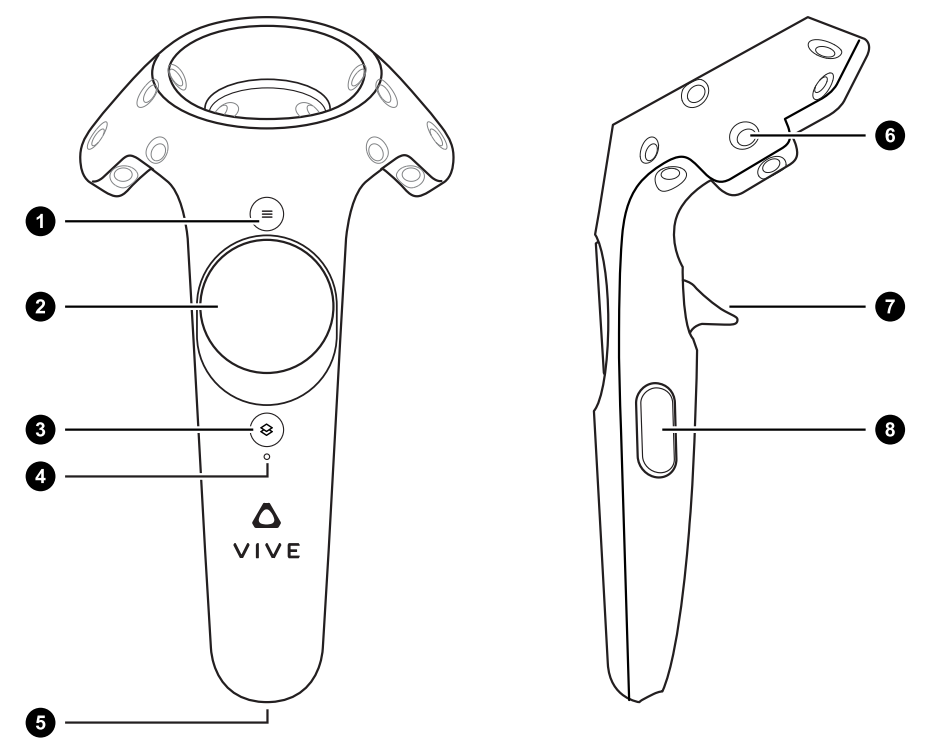
\includegraphics[width=10cm]{03_Figures/05_LitReview/HTCCorp2016_GestureController.png}
		\caption[Gesture Controller for the HTC Vive]{Gesture Controller for the HTC Vive \citep{HTCCorp2016}}
		\label{fig:gesturecontroller}
	\end{center}
\end{figure}


\subsubsection{Speech Recognition}

A system for the visualization of three-dimensional anatomical data, derived from magnetic resonance imaging (MRI) or computed tomography (CT), enables the physician to navigate through and interact with the patient's 3D scans in a virtual environment. This paper presents the multimodal human-machine interaction focusing the speech input. For the concerned task, a speech understanding front-end using a special kind of semantic decoder was successfully adopted
\cite{Muller1998}

The environment constructed in this research allows a user to communicate by talking and showing gestures
to a personified agent in virtual environment. A user can use his/her finger to point at a virtual object and ask the agent to manipulate the virtual object.
\cite{Uchino2008}

It allows user to interact with the virtual reality system with the static and stroke hand gesture along with speech. This multimodal interaction technique is able to perform few functions such as select, move, scale, rotate, copy, mirror, delete, check the shape, check and change the colour of an object.
\cite{Chun2015}


\subsubsection{Physical Placement of Interactive Objects}

Quite a bit older, from the 1990s, is the idea of dynamically placing physical knobs and switches in front of a seated user waring a HMD \citep{Latham1997}. The trajectory of the users hand and its movement is extrapolated in order to move the correct type of control in the right position just when it is expected in the virtual reality environment \citep{Latham1997}. Figure \ref{fig:touchcockpit} shows the concept of \cite{Latham1997} as well as how the final design looked like. Since such a machine requires a lot of time to design and build, it can be assumed that these are parts of the reason why not many further advancements were undertaken.
\begin{figure}[h]
	\begin{center}
		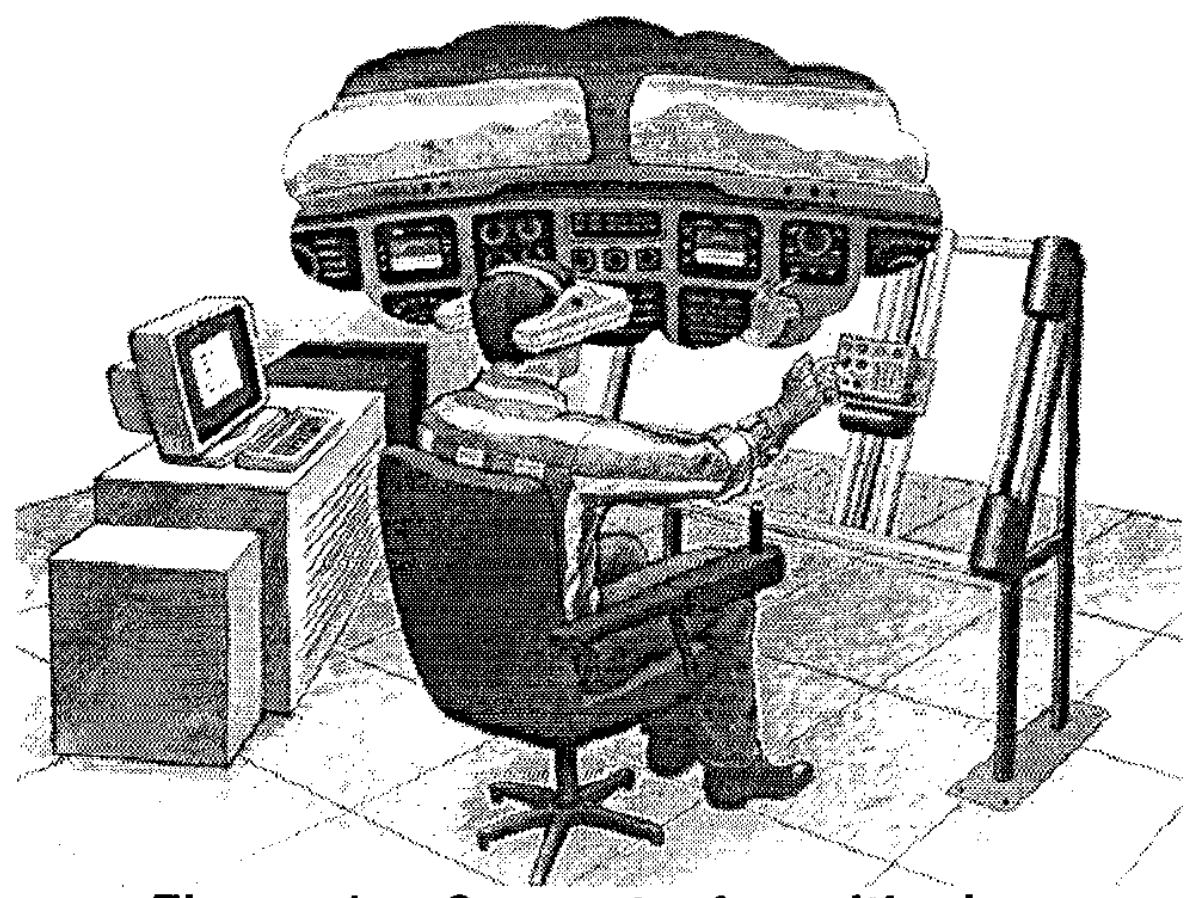
\includegraphics[width=6cm]{03_Figures/05_LitReview/Latham1997_Concept.png}
		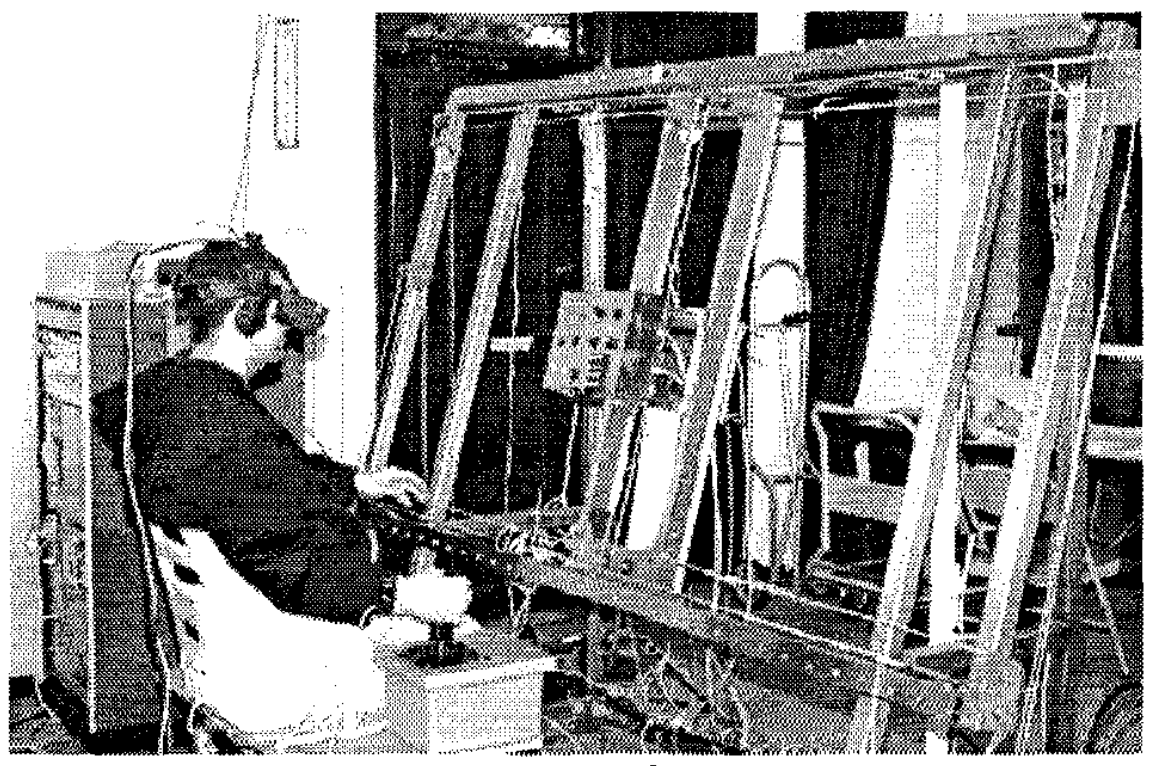
\includegraphics[width=7cm]{03_Figures/05_LitReview/Latham1997_FinalDesign.png}
		\caption[Concept and final design of positioning instrument controls to be touched in a virtual cockpit]{Concept (left) and final design (right) of positioning instrument controls to be touched in a virtual cockpit \citep{Latham1997}}
		\label{fig:touchcockpit}
	\end{center}
\end{figure}


\subsubsection{Full Body Tracking}

In June 2010, Microsoft announced the \textit{Kinect for Xbox 360}, a controller-free gaming device for the living room \citep{Microsoft2010}. Instead of relying on any physical input devices, the Kinect contains a comarea with motion-sensing technology that can track up to 48 points of movement on the human body, turning the player himself into a controller \citep{Microsoft2010}. \newline
Based on this technology, \cite{Takala2014} proposed a combination of a full body avatar controlled by Kinect with the Oculus Rift as display. This combination proved to be quite powerfull although they were facing a couple of challenges as well. The Kinect sometimes lost track of the hands or the movement was not recognized at all which \cite{Takala2014} tried to resolve by attaching a PlayStation Move to the HMD and put a Razer Hydra controller into the hands (Figure \ref{fig:kinectbody}). Although this improved the situation, different latencies of the individual dampened the experience. Furthermore, although Kinect was used for full-body tracking, only the movement of the hands and legs was utilized, whereas the movement within the virtual world was still relying on a physical controller.
\begin{figure}[h]
	\begin{center}
		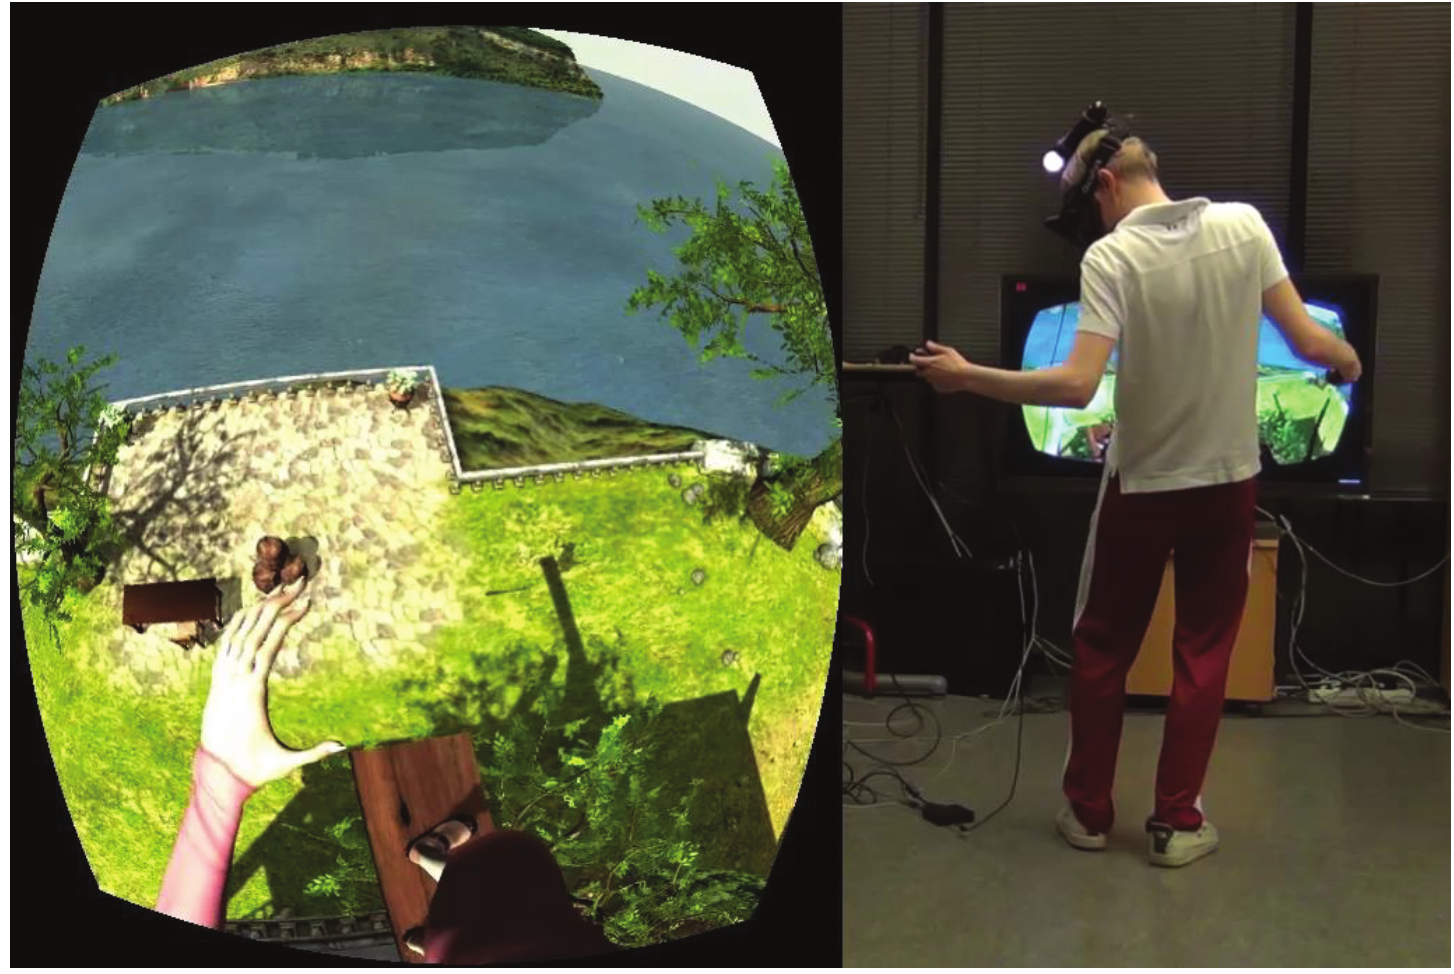
\includegraphics[width=12cm]{03_Figures/05_LitReview/Takala2014_KinectBody.png}
		\caption[Player's view of their virtual body that is tracked with Kinect]{Player's view of their virtual body (left) that is tracked with Kinect (right) \citep{Takala2014}}
		\label{fig:kinectbody}
	\end{center}
\end{figure}


\subsubsection{360° Motion Tracking}
\label{360MotionTracking}

One of the latest additions to the interaction possibilities is the 360° motion tracking, introduced with the HTC Vive which was just released in April 2016 \citep{Htcvive2016}. Figure \ref{fig:lighthouses} shows the setup of the two base stations (i.e. Lightouses) in opposing corners of the room that will be used for the 360° motion tracking. In essence, the two Lighthouse base stations emit a laser sweap across the room 60 times a second with a flash in between which allows any device with photosensors to calculate its exact position relative to the base station(s) \citep{Gizmodo2015}. This allows for a very accurate tracking and due to the opposing corners, at least one Lighthouse always has direct \textit{line of sight} to the HMD and the controllers. \newline
With this additional sensor information, the movement of the HMD and the controllers is tracked in all three axis and allow for new movements to be recognized, such as crouching or jumping within the relations of the room. \newline
So far there are no official devices that track the position of the feet, though this might only be a question of time.
\begin{figure}[h]
	\begin{center}
		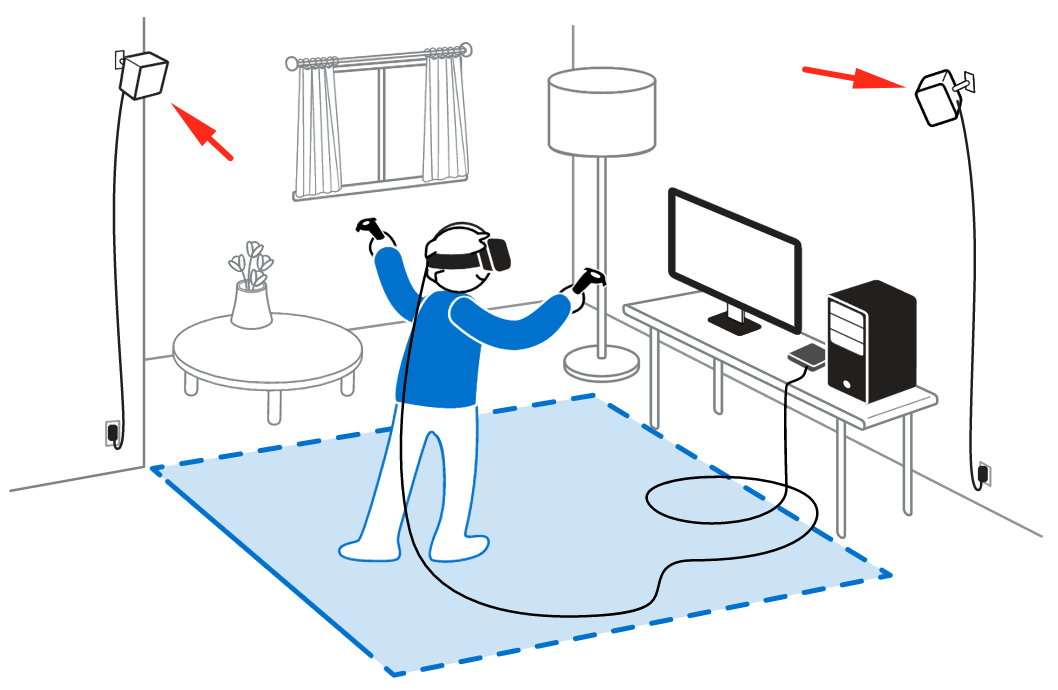
\includegraphics[width=10cm]{03_Figures/05_LitReview/HTCCorp2016_LighthouseRoomScale.png}
		\caption[Two Lighthouse in opposing corners allow for 360° motion tracking]{Two Lighthouse in opposing corners allow for 360° motion tracking \citep{HTCCorp2016}}
		\label{fig:lighthouses}
	\end{center}
\end{figure}

%-----------------------------------
%	SUBSECTION 3
%-----------------------------------

\subsection{Visual Information Seeking Mantra}

blub



%-----------------------------------
%	SUBSECTION 4
%-----------------------------------

\subsection{Conclusion}

blub



%----------------------------------------------------------------------------------------
%	SECTION 2
%----------------------------------------------------------------------------------------

\section{Existing Interaction Patterns with Virtual Reality}

\label{SectionLiteratureReviewSRQ2}

blub



%----------------------------------------------------------------------------------------
%	SECTION 3
%----------------------------------------------------------------------------------------

\section{Enhancement of Existing Interaction Patterns with new Methods for User Input}

\label{SectionLiteratureReviewSRQ3}

blub




%----------------------------------------------------------------------------------------
%	SECTION 4
%----------------------------------------------------------------------------------------

\section{Conclusion}

\label{SectionLiteratureReviewConclusion}

blub

